% !TEX encoding = UTF-8 Unicode
\documentclass{beamer}

\usepackage{color}
\usepackage{fancyvrb}
\usepackage{gensymb}
\usepackage{hyperref}
\usepackage{textcomp}
\usepackage{tikz}

\usetikzlibrary{arrows,positioning,shapes,shapes.multipart} 
\tikzstyle{every picture}+=[remember picture]

\definecolor{mygreen}{rgb}{0.88,0.95,0.88}

\usetheme{Warsaw}

\title[Data Visualization with R - Ggplot2 tutorial (part 1)]{Data Visualization with R \\ Ggplot2 tutorial (part 1)}
\author{Ariane Ducellier}
\date{University of Washington - Fall 2024}

\begin{document}

	\begin{frame}
		\titlepage
	\end{frame}

	\begin{frame}
		\frametitle{What is ggplot2?}

		Ggplot2 is the graphics package from the tidyverse, a collection of R packages designed for data science. 

		\vspace{2em}

		There is a base graphics package in R, which is present in the default version of R.

		\vspace{2em}

		However, ggplot2 gives users a lot more flexibility and control over their visualizations.
		
	\end{frame}

	\begin{frame}
		\frametitle{Main concepts of ggplot2}

		Ggplot2 is based on layers:

		\vspace{2em}
		
		\begin{itemize}
		\setlength{\itemsep}{1em}
			\item A first layer to describe the dataset.
			\item Layers describing the objects representing the data (dots, lines, bars, etc.).
			\item Additional objects describing the graphic itself (coordinates, scales, fonts, etc.).
		\end{itemize}

	\end{frame}

	\begin{frame}[fragile]
		\frametitle{Example: Histograms}

		Built-in R graphics package:

		\vspace{2em}

		\begin{exampleblock}{}
		\begin{center}
		\begin{BVerbatim}
hist(airquality$Temp)
		\end{BVerbatim}
		\end{center}
		\end{exampleblock}{}

		\vspace{2em}

		Quick plot using ggplot2:

		\vspace{2em}

		\begin{exampleblock}{}
		\begin{center}
		\begin{BVerbatim}
qplot(airquality$Temp)
		\end{BVerbatim}
		\end{center}
		\end{exampleblock}{}

	\end{frame}

	\begin{frame}[fragile]
		\frametitle{Ggplot2 command structure}

		\begin{exampleblock}{}
		\begin{center}
		\begin{BVerbatim}
ggplot(airquality, aes(x=Temp))
		\end{BVerbatim}
		\end{center}
		\end{exampleblock}{}

		\vspace{2em}

		\begin{center}
		This command does not plot anything.
		\end{center}

		\vspace{2em}

		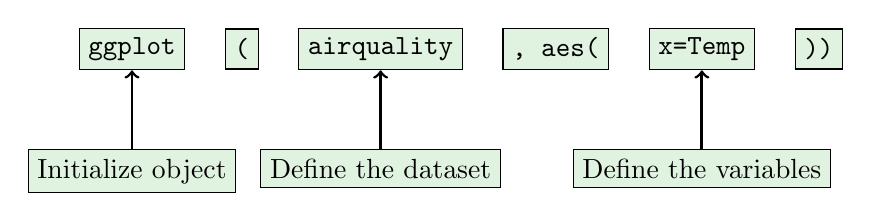
\begin{tikzpicture}
			\node[align=center, draw, rectangle, fill=mygreen] (l1) {
				\begin{BVerbatim}
ggplot
				\end{BVerbatim}
			};
			\node[right=0.5cm of l1] (l2) [align=center, draw, rectangle, fill=mygreen] {
				\begin{BVerbatim}
(
				\end{BVerbatim}
			};
			\node[right=0.5cm of l2] (l3) [align=center, draw, rectangle, fill=mygreen] {
				\begin{BVerbatim}
airquality
				\end{BVerbatim}
			};
			\node[right=0.5cm of l3] (l4) [align=center, draw, rectangle, fill=mygreen] {
				\begin{BVerbatim}
, aes(
				\end{BVerbatim}
			};
			\node[right=0.5cm of l4] (l5) [align=center, draw, rectangle, fill=mygreen] {
				\begin{BVerbatim}
x=Temp
				\end{BVerbatim}
			};
			\node[right=0.5cm of l5] (l6) [align=center, draw, rectangle, fill=mygreen] {
				\begin{BVerbatim}
))
				\end{BVerbatim}
			};

			\node[below=1cm of l1] (l7) [align=center, draw, rectangle, fill=mygreen] {Initialize object};
			\node[below=1cm of l3] (l8) [align=center, draw, rectangle, fill=mygreen] {Define the dataset};
			\node[below=1cm of l5] (l9) [align=center, draw, rectangle, fill=mygreen] {Define the variables};

			\path[draw,->, line width=1pt] (l7.north) -- node[above=0.5cm,left] {} (l1.south);
			\path[draw,->, line width=1pt] (l8.north) -- node[below=0.5cm,left] {} (l3.south);
			\path[draw,->, line width=1pt] (l9.north) -- node[above=0.5cm,left] {} (l5.south);
		\end{tikzpicture}

	\end{frame}

	\begin{frame}[fragile]
		\frametitle{Ggplot2 command structure}

		We need to add a command to explain the kind of object that we want to plot:

		\vspace{2em}

		\begin{exampleblock}{}
		\begin{BVerbatim}
ggplot(airquality, aes(x=Temp)) +
geom_histogram()
		\end{BVerbatim}
		\end{exampleblock}{}
		
	\end{frame}

	\begin{frame}[fragile]
		\frametitle{Bar plots}

		We can use bar plots to visualize one categorical variable:

		\vspace{2em}

		\begin{exampleblock}{}
		\begin{BVerbatim}
ggplot(df_desc, aes(x=Vancouver)) +
geom_bar()
		\end{BVerbatim}
		\end{exampleblock}{}

		\vspace{2em}

		The height of the bar is proportional to the number of cases in each group.
		
	\end{frame}

	\begin{frame}[fragile]
		\frametitle{Bar plots}

		Or a combination of a categorical variable and a continuous variable:

		\vspace{2em}

		\begin{exampleblock}{}
		\begin{BVerbatim}
ggplot(RetailSales, aes(x=Month, y=Sales)) + 
geom_bar(stat="identity")
		\end{BVerbatim}
		\end{exampleblock}{}

		\vspace{2em}

		Using \verb|stat = "identity"| tells ggplot2 to sum the values for each group (Month) and plot bars proportional to the sums.
		
	\end{frame}

	\begin{frame}[fragile]
		\frametitle{Box plots}

		For each layer that we want to add on our plot, we add the corresponding object:

		\vspace{2em}

		\begin{exampleblock}{}
		\begin{BVerbatim}
ggplot(df_hum, aes(x=month, y=Vancouver)) + 
geom_boxplot()
		\end{BVerbatim}
		\end{exampleblock}{}
		
	\end{frame}

	\begin{frame}[fragile]
		\frametitle{Scatter plots and line plots}

		The relationship between two continuous variables can be visualize with a scatter plot or a line plot:

		\vspace{2em}

		\begin{exampleblock}{}
		\begin{BVerbatim}
ggplot(df, aes(x=time, y=distance)) +
geom_point()
		\end{BVerbatim}
		\end{exampleblock}{}

		\vspace{2em}

		\begin{exampleblock}{}
		\begin{BVerbatim}
ggplot(df, aes(x=time, y=distance)) +
geom_line()
		\end{BVerbatim}
		\end{exampleblock}{}
		
	\end{frame}

	\begin{frame}[fragile]
		\frametitle{Changing histogram defaults}

		Modify the number of bins:

		\vspace{2em}

		\begin{exampleblock}{}
		\begin{BVerbatim}
ggplot(df_hum, aes(x=Vancouver)) + 
geom_histogram(bins=15)
		\end{BVerbatim}
		\end{exampleblock}{}

		\vspace{2em}

		Modify the filling and the color:

		\vspace{2em}

		\begin{exampleblock}{}
		\begin{BVerbatim}
ggplot(df_hum, aes(x=Vancouver)) + 
geom_histogram(bins=15, fill="white", color=1)
		\end{BVerbatim}
		\end{exampleblock}{}
	\end{frame}

	\begin{frame}[fragile]
		\frametitle{Adding aesthetics to the plot}

		Add title and axis labels to the histogram:

		\vspace{2em}

		\begin{exampleblock}{}
		\begin{BVerbatim}
ggplot(df_hum, aes(x=Vancouver)) + 
geom_histogram(bins=15, fill="white", color=1) +
ggtitle("Humidity for Vancouver city") +
xlab("Humidity") +
theme(axis.text.x=element_text(size=12),
axis.text.y=element_text(size=12))
		\end{BVerbatim}
		\end{exampleblock}{}
		
	\end{frame}

	\begin{frame}[fragile]
		\frametitle{Adding aesthetics to the boxplot}

		Add labels to the box plot:

		\vspace{2em}

		\begin{exampleblock}{}
		\begin{BVerbatim}
ggplot(df_hum, aes(x=month, y=Vancouver)) + 
geom_boxplot(color=1, fill=3) + 
ylab("Humidity") + 
theme(axis.text.x=element_text(size=15),
axis.text.y=element_text(size=15),
axis.title.x=element_text(size=15, color=2),
axis.title.y=element_text(size=15, color=2))
		\end{BVerbatim}
		\end{exampleblock}{}
		
	\end{frame}

\end{document}
